\documentclass{article}
\usepackage{tikz}
\usepackage{float}
\usepackage{lmodern}
\usepackage{amsmath}
\usepackage{xcolor}
\usetikzlibrary{calc}
\usetikzlibrary{shapes}
\usetikzlibrary{decorations.markings, decorations.pathreplacing}

\begin{document}

\centering

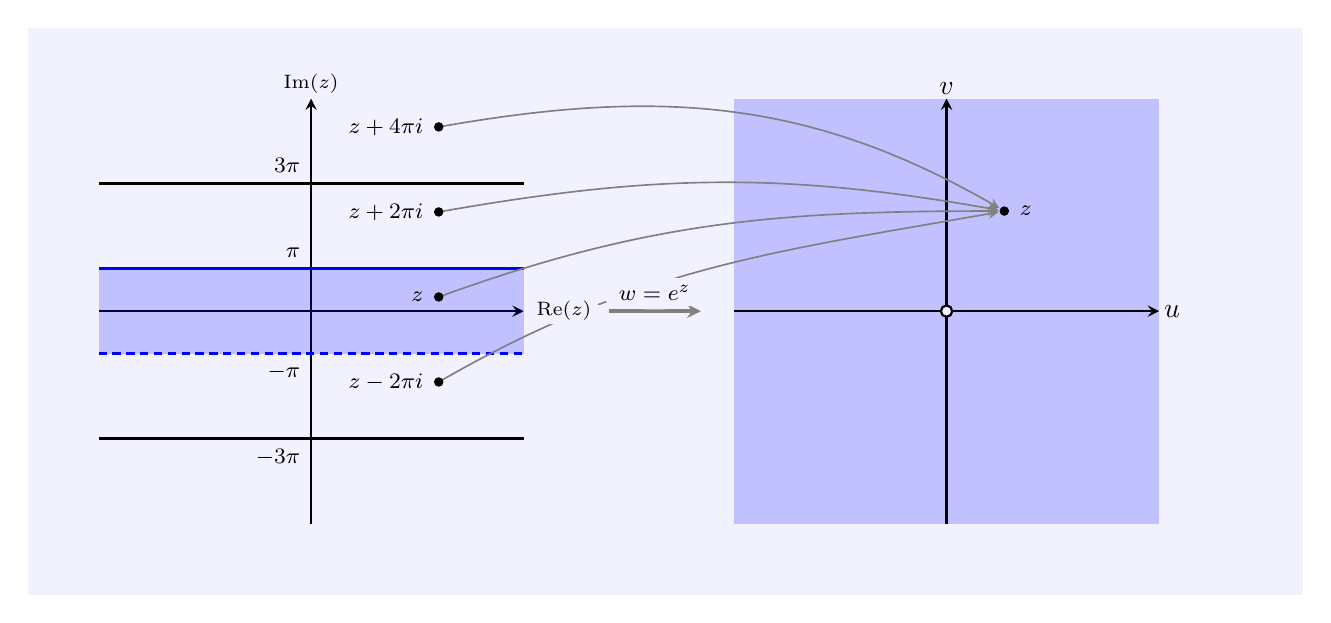
\begin{tikzpicture}[scale=0.9]
% conversion from cm to pt and vice versa
\pgfmathsetmacro{\CmToPt}{28.3464566929}
\pgfmathsetmacro{\PtToCm}{0.0352777778}
% define styles used in this picture
\pgfmathsetmacro{\CircleSize}{0.03}         % radius of coordinate circles/dots
\tikzset{
BigTextFont/.style={font=\normalsize},              % Big text font
every node/.style={font=\footnotesize,text=black},  % Small text font
CircleNodeStyle/.style={draw=black, shape=circle, fill=black, minimum size=\CircleSize*2.5 cm, inner sep=0pt},
every path/.style={very thick},
arrowstyle/.style={->, >=stealth}}

\colorlet{BlueBackground}{blue!5}
% Background for entire canvas
\fill[BlueBackground] (-4.0,-4.0) rectangle (14.0,4.0);

% custom colors
\definecolor{ContourHighlight}{rgb}{255,0,0}        % color to highlight contours of the function
\definecolor{BlueDomain}{rgb}{0, 0, 128}

% control dimensions of filled area in domain of function
\pgfmathsetmacro{\AreaWidth}{3.0}
\pgfmathsetmacro{\AreaHeight}{\AreaWidth}

% define layers
\pgfdeclarelayer{foreground}
\pgfsetlayers{main,foreground}

%% AXES
% function for drawing axes complex plane
\newcommand{\DrawComplexAxes}[4]{%
  \pgfmathsetmacro{\AxisSizeX}{#1}
  \pgfmathsetmacro{\AxisSizeY}{#2}

  % Draw axes
  \draw[arrowstyle, thick]  
    (-\AxisSizeX/2, 0) -- (\AxisSizeX/2, 0);
  \draw[arrowstyle, thick] 
    (0, -\AxisSizeY/2) -- (0, \AxisSizeY/2);

  % Foreground labels
  \begin{pgfonlayer}{foreground}
    \node[ellipse, fill=BlueBackground, right, inner sep=0pt, font=\scriptsize] 
      at (\AxisSizeX/2, 0) {#3};
    \node[ellipse, fill=BlueBackground, above, inner sep=0pt, font=\scriptsize] 
      at (0, \AxisSizeY/2) {#4};
  \end{pgfonlayer}
}

\DrawComplexAxes{\AreaWidth * 2}{\AreaHeight * 2}{$\mathrm{Re}(z)$}{$\mathrm{Im}(z)$}

% variables for spacing in the complex grid
\pgfmathsetmacro{\YTickscaling}{\AreaHeight * 0.2}
\pgfmathsetmacro{\XTickscaling}{1.8}
\pgfmathsetmacro{\Ticksize}{0.1}

% draw the filled area and its borders
\pgfmathsetmacro{\FilledAreaHeight}{\YTickscaling}
\fill[color=BlueDomain, opacity=0.2] (-\AreaWidth, -\FilledAreaHeight) -- (\AreaWidth, -\FilledAreaHeight) -- (\AreaWidth, \FilledAreaHeight) -- (-\AreaWidth, \FilledAreaHeight) -- cycle;
\draw[color=BlueDomain, densely dashed] (-\AreaWidth, -\FilledAreaHeight) -- (\AreaWidth, -\FilledAreaHeight);
\draw[color=BlueDomain] (\AreaWidth, \FilledAreaHeight) -- (-\AreaWidth, \FilledAreaHeight);

% draw y-ticks
\node[above left] at (0, 1*\YTickscaling) {$\pi$};
\node[below left] at (0, -1*\YTickscaling) {$-\pi$};
\node[above left] at (0, 3*\YTickscaling) {$3 \pi$};
\node[below left] at (0, -3*\YTickscaling) {$-3 \pi$};

% draw area separations
\draw (\AreaWidth, 3*\YTickscaling) -- (-\AreaWidth, 3*\YTickscaling);
\draw (\AreaWidth, -3*\YTickscaling) -- (-\AreaWidth, -3*\YTickscaling);

%% Draw the points in the domain
\pgfmathsetmacro{\XCoord}{1.0}
\pgfmathsetmacro{\YCoord}{pi/3}

\begin{scope}[xscale = \XTickscaling, yscale = \YTickscaling / pi]
    % define the coordinates
    \coordinate (FundamentalPoint) at (\XCoord, \YCoord);
    \coordinate (PointPlusOne) at ($(FundamentalPoint) + (0.0, 2*pi)$);
    \coordinate (PointPlusTwo) at ($(FundamentalPoint) + (0.0, 4*pi)$);
     \coordinate (PointMinOne) at ($(FundamentalPoint) + (0.0, -2*pi)$);

\end{scope}



%% 2ND PLOT: range of the function

% define scaling in range of function
\pgfmathsetmacro{\SecondPlotScale}{0.6}



\begin{scope}[xshift = \AreaWidth * 3 * \CmToPt]
% background for subcanvas 
  \pgfmathsetmacro{\BackgroundSize}{\AreaWidth*1.0}
  \fill[color=BlueDomain, opacity=0.2] (-\BackgroundSize, -\BackgroundSize) rectangle (\BackgroundSize, \BackgroundSize);

  % draw axes
  \DrawComplexAxes{\AreaWidth * 2}{\AreaWidth * 2}{\normalsize $u$}{\normalsize $v$}

  % draw point in the range of the function
  \pgfmathsetmacro{\ExpRadius}{exp(\XCoord) * \YTickscaling}
  \pgfmathsetmacro{\AngleDeg}{\YCoord * 180/pi}
  \coordinate (ValuePoint) at (\AngleDeg: \ExpRadius);
  \node[CircleNodeStyle, label=right:{$z$}] (ValuePointNode) at (ValuePoint) {};

  % draw small circle to indicate that 0 is not part of the range of the function
  \draw[fill=BlueBackground, draw=black, thick] (0,0) circle [radius=0.08];
\end{scope}

\tikzset{
  MyArrowStyle/.style={
    arrowstyle,
    semithick,
    gray,
    shorten >=0.5pt
  }
}

% draw arrows from the points in the domain to the point in the range of the function
\draw[MyArrowStyle] (FundamentalPoint)  to[out=20,in=180] (ValuePointNode);
\draw[MyArrowStyle] (PointPlusOne)  to[out=10,in=180-10] (ValuePointNode);
\draw[MyArrowStyle] (PointPlusTwo)  to[out=10,in=180-30] (ValuePointNode);
\draw[MyArrowStyle] (PointMinOne)  to[out=30,in=180+10] (ValuePointNode);

 % draw coordinates of the points in the domain
\node[CircleNodeStyle, label=left:{$z$}] at (FundamentalPoint) {};
\node[CircleNodeStyle, label=left:{$z + 2 \pi i$}] at (PointPlusOne) {};
\node[CircleNodeStyle, label=left:{$z + 4 \pi i$}] at (PointPlusTwo) {};
\node[CircleNodeStyle, label=left:{$z - 2 \pi i$}] at (PointMinOne) {};

% arrow for the function
\draw[arrowstyle, color=gray, postaction={decorate}, 
    decoration={markings, mark=at position 0.5 with {\node[above, ellipse, fill=BlueBackground, inner sep=1.5pt] {$w = e^{z}$};}}]
     (\AreaWidth + 1.2, 0.0) -- (2*\AreaWidth - 0.5, 0.0);

\end{tikzpicture}

\end{document}